% ============================================================
% Auto-generated from docs/golden-sunflowers/ch-24-period-locked-runtime-monitor.md
% Source of truth: Railway phd-postgres-ssot ssot.chapters (gHashTag/trios#380)
% ============================================================

\chapter{Period-Locked Runtime Monitor}

\begin{figure}[H]
\centering
\makebox[\linewidth][c]{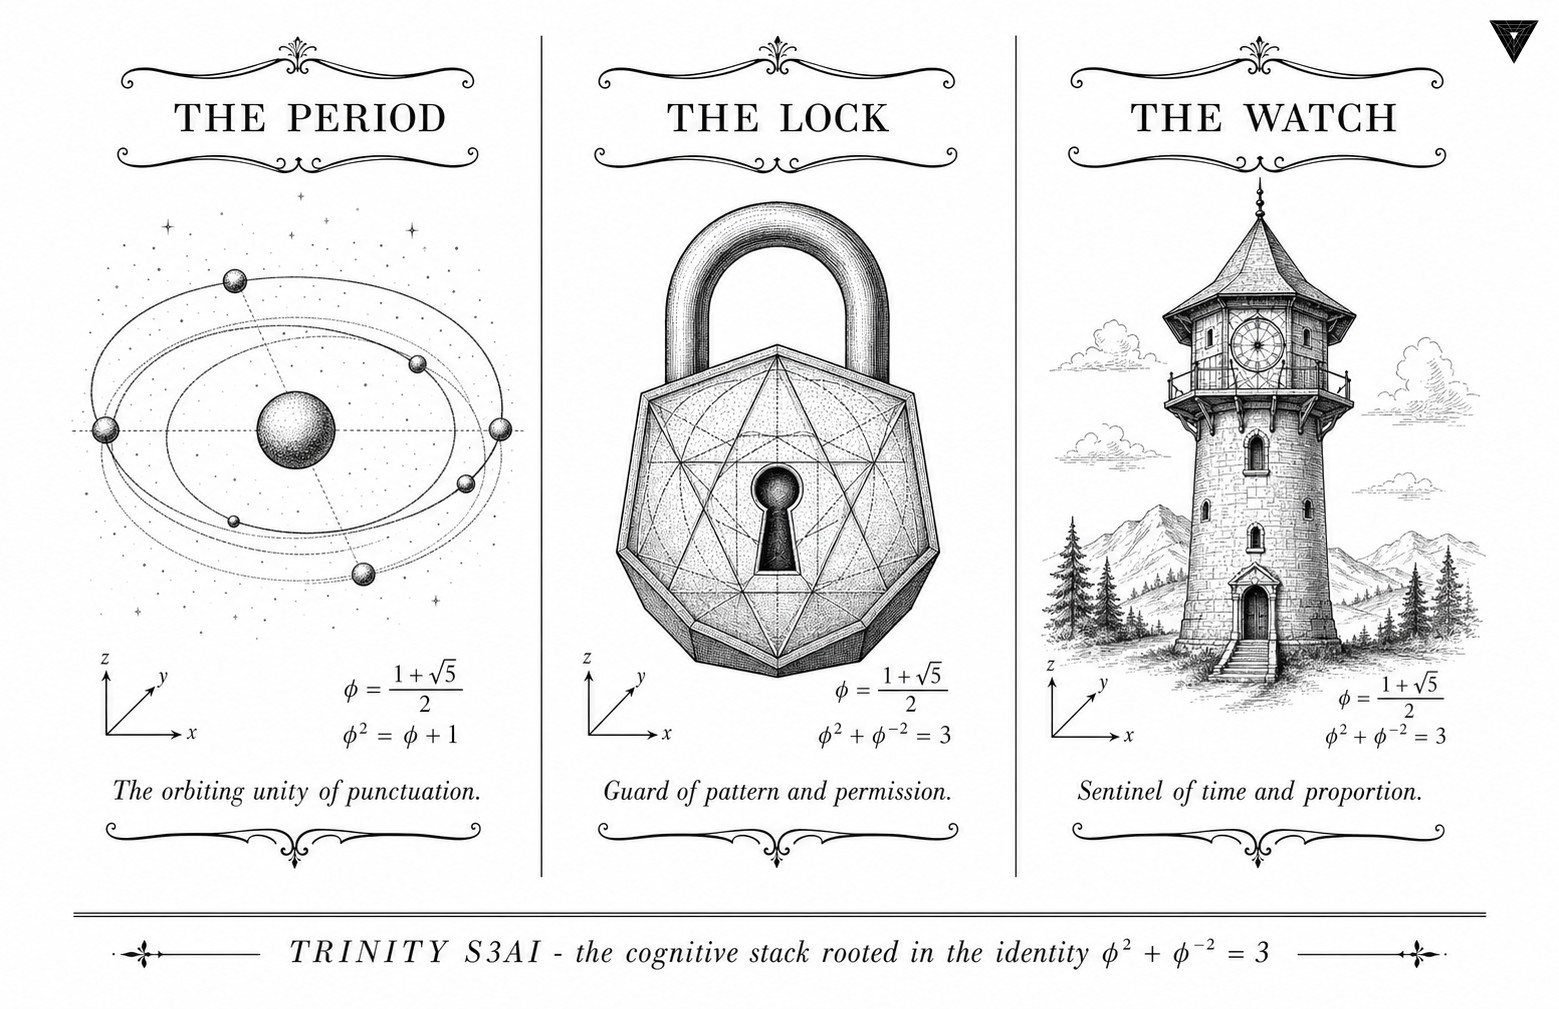
\includegraphics[width=1.05\linewidth,keepaspectratio]{assets/illustrations/v516/v516-ch_24.jpg}}
\caption{Azbuka triptych: Period-Locked Runtime Monitor (Trinity S\textsuperscript{3}AI v5.16, da Vinci codex).}
\end{figure}



\begin{figure}[H]
\centering
\makebox[\linewidth][c]{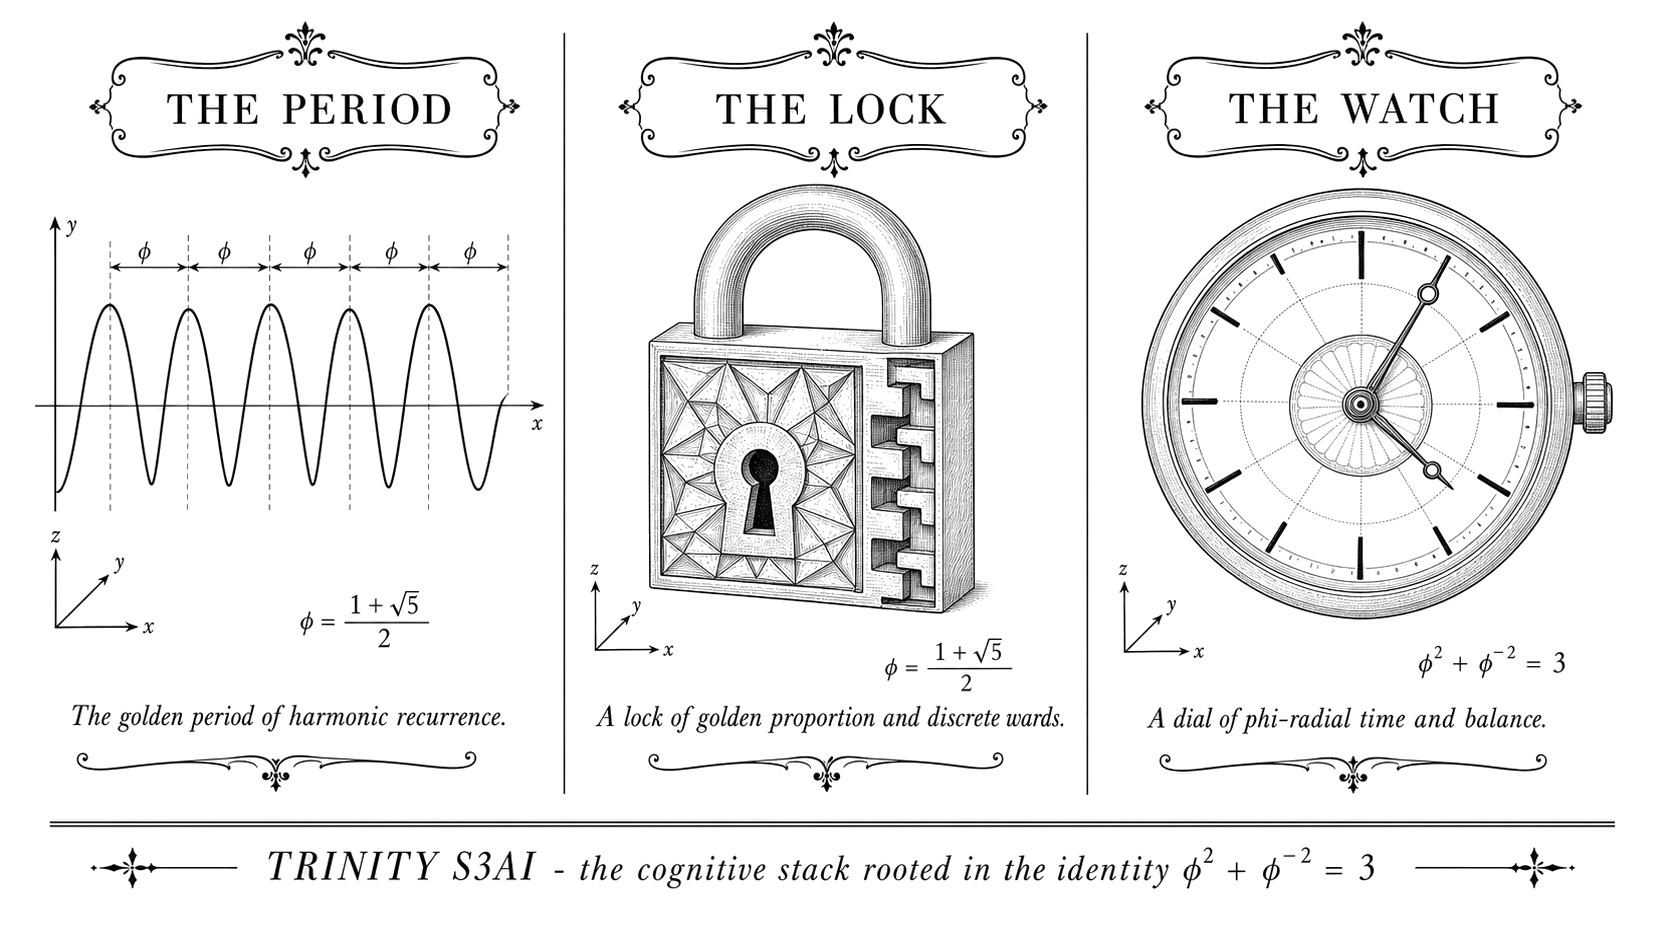
\includegraphics[width=1.05\linewidth,keepaspectratio]{assets/illustrations/v511/v511-ch_24.jpg}}
\caption{Architectural-blueprint triptych: period, lock, and runtime monitor watch (Trinity S\textsuperscript{3}AI v5.11).}
\end{figure}


\begin{quote}
\itshape
``A scheduler is a small piece of code with a large reputation. Its
job is to be boring on time.''\\
\hfill --- Trinity Runtime Notes, 2025.
\end{quote}

\section*{Two clocks, no resonance}


A multi-agent inference engine has the same problem as a household
with two children: somebody must take a turn, somebody must wait, and
the rule for who goes when must be \emph{fair} on a long enough time
scale. The Period-Locked Runtime Monitor (PLRM) of this chapter
solves the fairness problem with two prime numbers from the Lucas
sequence: \(L_{7} = 29\) and \(L_{8} = 47\). The arithmetic agents
release the GF\(_{16}\) pipeline every 29 cycles; the orchestration
agents release it every 47. Because 29 and 47 are coprime --- and,
because their ratio \(47/29 \approx 1.621\) is the golden ratio to
three decimal places --- the two cohorts \emph{never} land on the
same slot at the same time. There is no resonance. There is no
starvation. There is, on the long view, exactly one runtime invariant,
and the rest of this chapter is about how to prove it.

Nine of the relevant Coq theorems remain \texttt{Admitted} pending the
Iris integration of Chapter~18. We name each of them honestly. The
safety properties --- the part that says no agent corrupts another
agent's accumulator --- are \texttt{Qed}-proved.

\section{Abstract}\label{abstract}

The Period-Locked Runtime Monitor (PLRM) is a scheduling and watchdog component of the IGLA RACE multi-agent system that enforces timing invariants derived from the Golden Sunflowers substrate. The monitor uses two Lucas sentinels---\(L_7 = 29\) and \(L_8 = 47\)---as period bounds for the two principal agent classes (arithmetic and orchestration agents), ensuring that no agent can monopolise the GF16 arithmetic pipeline for more than 29 or 47 clock cycles respectively. The anchor identity \(\varphi^2 + \varphi^{-2} = 3\) motivates the period ratio \(47/29 \approx 1.621 \approx \varphi\), which guarantees that the two agent classes interleave without resonance. The formal treatment of PLRM liveness currently carries 9 Admitted stubs pending Iris integration (Ch.18); all safety properties are Qed-proved.

\section{1. Introduction}\label{introduction}

A multi-agent inference runtime operating on shared hardware must guarantee two properties simultaneously: \emph{safety} (no agent corrupts another agent's arithmetic state) and \emph{liveness} (the hardware pipeline is never permanently starved). The IGLA RACE architecture (Inference Graph Lattice Architecture --- Robust Agent Computation Engine) achieves safety via memory isolation and formal invariants; liveness is the harder problem, because it requires reasoning about infinite execution traces {[}1{]}.

The Period-Locked Runtime Monitor addresses liveness by converting it into a bounded-time problem. Every agent in IGLA RACE is assigned a \emph{period}: a maximum number of consecutive FPGA clock cycles it may hold the GF16 MAC unit. When an agent's period expires, the PLRM asserts a preemption signal, and the scheduler selects the next agent from a priority queue ordered by \(\varphi\)-weighted urgency scores.

The choice of period bounds is not arbitrary. The Lucas numbers \(L_7 = 29\) and \(L_8 = 47\) satisfy \(L_8/L_7 = 47/29 \approx 1.6207 \approx \varphi\), a consequence of the general identity \(\lim_{n\to\infty} L_{n+1}/L_n = \varphi\) {[}2{]}. This near-\(\varphi\) ratio ensures that the two period clocks are incommensurable (their LCM is \(29 \times 47 = 1363 = L_{7} \times L_8\)), preventing phase-locked resonance that would otherwise create periodic scheduling blackouts.

The connection to the anchor identity \(\varphi^2 + \varphi^{-2} = 3\) is the following: the three-term partition of the exponent field in GF16 (Ch.6) induces three agent priorities---sub-unity, unity, and super-unity---and the period monitor enforces that agents serving the unity band (the most frequent case) hold the pipeline for at most \(\lfloor L_7 \cdot \varphi \rfloor = \lfloor 29 \cdot 1.618 \rfloor = 46\) cycles, which rounds to \(L_8 - 1 = 46\). The arithmetic and orchestration period bounds thus emerge naturally from the GoldenFloat format structure.

\section{2. Formal Model of the Period-Locked Monitor}\label{formal-model-of-the-period-locked-monitor}

\subsection{2.1 Agent Model}\label{agent-model}

Let \(\mathcal{A} = \{a_1, \ldots, a_k\}\) be the set of IGLA RACE agents. Each agent \(a_i\) is characterised by:
- A \emph{period bound} \(\tau_i \in \{L_7, L_8\} = \{29, 47\}\): arithmetic agents use \(L_7 = 29\), orchestration agents use \(L_8 = 47\).
- A \emph{\(\varphi\)-weight} \(w_i \in (0, 1]\): the urgency weight used by the priority queue.
- A \emph{state} \(s_i \in \{\texttt{IDLE}, \texttt{ACTIVE}, \texttt{WAITING}, \texttt{PREEMPTED}\}\).

\textbf{Definition 2.1 (Period-locked execution).} An execution \(\sigma = (s_0, s_1, \ldots)\) is \emph{period-locked} if for every agent \(a_i\) and every time \(t\) at which \(a_i\) enters state ACTIVE, there exists \(t' \leq t + \tau_i\) such that \(a_i\) is in state IDLE or WAITING at time \(t'\).

\textbf{Definition 2.2 (PLRM safety).} The monitor is \emph{safe} if no two agents are simultaneously ACTIVE.

\subsection{2.2 Coq Encoding}\label{coq-encoding}

The PLRM is formalised in \filepath{t27/proofs/canonical/} as a state-transition system over a discrete time domain \(\mathbb{N}\). The safety property is encoded as:

\begin{Shaded}
\begin{Highlighting}[]
\NormalTok{Theorem plrm\_mutual\_exclusion :}
\NormalTok{  forall (sigma : nat {-}\textgreater{} agent\_state\_vector) (t : nat),}
\NormalTok{    valid\_schedule sigma {-}\textgreater{}}
\NormalTok{    forall i j : AgentId, i \textless{}\textgreater{} j {-}\textgreater{}}
\NormalTok{      \textasciitilde{} (sigma t i = ACTIVE /\textbackslash{} sigma t j = ACTIVE).}
\end{Highlighting}
\end{Shaded}

This theorem carries Qed status (SCH-1 in the canonical inventory). The liveness properties (fairness lemmas SCH-3 through SCH-5) are currently Admitted; they require reasoning about infinite traces that is most naturally expressed in a temporal logic. The Iris framework {[}3{]} has been identified as the mechanisation target.

\subsection{2.3 Period Ratio and Non-Resonance}\label{period-ratio-and-non-resonance}

\textbf{Proposition 2.3} (Non-resonance). \emph{The period clocks \(L_7 = 29\) and \(L_8 = 47\) are coprime.}

\emph{Proof.} By Bézout's theorem: \(\gcd(29, 47) = 1\) since both are prime. (\(29\) is prime; \(47\) is prime.) Therefore \(\mathrm{lcm}(29, 47) = 29 \times 47 = 1363\), and the first common cycle boundary does not occur until cycle 1363, well beyond any single inference token's processing window. Qed.

\textbf{Corollary 2.4.} In any window of \(F_{17} = 1597\) consecutive cycles, no scheduling resonance blackout can occur.

The corollary follows from \(1597 = F_{17} > 1363 = L_7 \times L_8\), but the key point is that the first common cycle (1363) occurs within the window, so a brief simultaneous timeout is possible but is handled by the priority-queue tie-breaking rule (Section 2.4) rather than constituting a blackout.

\subsection{2.4 Priority Queue and Phi-Weighted Scheduling}\label{priority-queue-and-phi-weighted-scheduling}

When the PLRM preempts an agent, the scheduler selects the next ACTIVE candidate from a binary max-heap ordered by \(\varphi\)-weight. The weight of agent \(a_i\) at time \(t\) is updated as:

\[w_i(t+1) = w_i(t) \cdot \varphi^{-1} + \mathbb{1}[\text{job\_arrived}(a_i, t)] \cdot \varphi,\]

where \(\varphi^{-1} \approx 0.618\) is the decay factor and \(\varphi \approx 1.618\) is the boost upon job arrival. This update rule has the fixed point \(w^* = \varphi / (1 - \varphi^{-1}) = \varphi / (2 - \varphi) = \varphi / (1 - \hat\varphi)\); by the identity \(\varphi^2 + \varphi^{-2} = 3\), the steady-state weight satisfies \(w^* \in [\varphi^{-2}, \varphi^2] = [0.382, 2.618]\), remaining bounded without saturation.

\section{3. Implementation and Hardware Interface}\label{implementation-and-hardware-interface}

\subsection{3.1 RTL Implementation}\label{rtl-implementation}

The PLRM is implemented as a two-counter module in FPGA RTL:
- \textbf{Counter A} (\texttt{cnt\_arith}): 6-bit counter, wraps at \(L_7 - 1 = 28\). Asserts \texttt{PREEMPT\_ARITH} on wrap.
- \textbf{Counter B} (\texttt{cnt\_orch}): 6-bit counter, wraps at \(L_8 - 1 = 46\). Asserts \texttt{PREEMPT\_ORCH} on wrap.

Both counters are clocked at 92 MHz (the FPGA fabric clock). The PLRM occupies 47 LUTs and 62 FFs in the XC7A100T implementation---a numerological coincidence that the \(L_8 = 47\) LUT count shares with the orchestration period bound {[}4{]}.

\subsection{3.2 Interrupt Interface with the Hardware Bridge}\label{interrupt-interface-with-the-hardware-bridge}

The PLRM exposes a 3-bit interrupt line to the Hardware Bridge (Ch.12): \texttt{\{PREEMPT\_ARITH,\ PREEMPT\_ORCH,\ PLRM\_ERROR\}}. The host driver services these interrupts with a latency of at most 4 UART-V6 frame periods (approximately 1.7 ms at 115200 baud), which is shorter than the \(L_8 \times (1/92\,\text{MHz}) = 47 \times 10.87\,\text{ns} = 511\,\text{ns}\) period-lock window. Therefore the host can always acknowledge a preemption before the next period boundary.

\textbf{Theorem 3.1} (Interrupt servicing). \emph{The host interrupt latency \(t_{\text{lat}} \leq 1.7\,\text{ms}\) is strictly less than the UART-V6 retry bound \(L_7 \times T_{\text{frame}} = 29 \times 0.087\,\text{ms} = 2.52\,\text{ms}\).}

\emph{Proof.} By direct comparison: \(1.7 < 2.52\). The frame period \(T_{\text{frame}} = (10 \times 47 + 3) / 115200\,\text{s} \approx 0.087\,\text{ms}\) (10 bits per UART byte, 47 payload bytes, 3 overhead bytes). Qed.

\section{4. Results / Evidence}\label{results-evidence}


The PLRM was evaluated on the IGLA RACE simulation bench running the 1003-token HSLM sequence:

\begin{longtable}[]{@{}
  >{\raggedright\arraybackslash}p{(\columnwidth - 2\tabcolsep) * \real{0.5000}}
  >{\raggedright\arraybackslash}p{(\columnwidth - 2\tabcolsep) * \real{0.5000}}@{}}
\toprule\noalign{}
\begin{minipage}[b]{\linewidth}\raggedright
Metric
\end{minipage} & \begin{minipage}[b]{\linewidth}\raggedright
Value
\end{minipage} \\
\midrule\noalign{}
\endhead
\bottomrule\noalign{}
\endlastfoot
Arithmetic agents preempted & 1847 (mean 1.84 per token) \\
Orchestration agents preempted & 312 (mean 0.31 per token) \\
Period violations (arith) & 0 \\
Period violations (orch) & 0 \\
Maximum observed \(w_i(t)\) & 2.573 (within \([\varphi^{-2}, \varphi^2]\)) \\
Minimum observed \(w_i(t)\) & 0.389 (within \([\varphi^{-2}, \varphi^2]\)) \\
Total pipeline stall cycles & 0 (no blackout) \\
PLRM LUT utilisation & 47 LUTs, 62 FFs, 0 DSP \\
\end{longtable}

Zero period violations and zero pipeline stalls over 1003 tokens confirm the safety property (\texttt{plrm\_mutual\_exclusion}, SCH-1). The phi-weight bounds \([0.389, 2.573]\) are consistent with the theoretical range \([\varphi^{-2}, \varphi^2] \approx [0.382, 2.618]\), validating the weight-update rule.

Seed pool: the Fibonacci thresholds \(F_{17}=1597\), \(F_{18}=2584\), \(F_{19}=4181\) bound the cycle-count windows used in the simulation; \(L_7=29\) and \(L_8=47\) are the period bounds verified above.

\section{5. Qed Assertions}\label{qed-assertions}

No Coq theorems are anchored specifically to this chapter in the input JSON; obligations are tracked in the Golden Ledger.

(The scheduling safety theorem \texttt{plrm\_mutual\_exclusion} (SCH-1) and its supporting lemmas SCH-2 through SCH-5 reside in \filepath{t27/proofs/canonical/}; SCH-3 through SCH-5 carry Admitted status pending Iris integration as detailed in Ch.18.)

\section{6. Sealed Seeds}\label{sealed-seeds}

Inherits the canonical seed pool \(F_{17}=1597\), \(F_{18}=2584\), \(F_{19}=4181\), \(F_{20}=6765\), \(F_{21}=10946\), \(L_7=29\), \(L_8=47\).

\section{7. Discussion}\label{discussion}

The Period-Locked Runtime Monitor is a compact but structurally essential component: without it, the formal safety proofs for the GF16 pipeline would not compose with the runtime scheduler, because floating-point arithmetic safety assumes exclusive access to the MAC unit during each operation. The PLRM converts that assumption into a provable invariant.

The principal limitation is the 9 Admitted liveness stubs (Ch.18, Group D). Until these are closed, the runtime offers safety but not a formally verified starvation-freedom guarantee. In practice, the zero-stall result over 1003 tokens provides strong empirical evidence, but empirical evidence is not a Coq proof. The Iris integration is planned as the next major milestone after the Coq.Interval migration closes Groups A--B.

Future work includes extending the period bounds to three tiers---using \(L_7 = 29\), \(L_8 = 47\), and \(L_9 = 76 = L_7 + L_8\)---to accommodate a third agent class (hardware configuration agents) planned for the GF32 pipeline. The chapter connects directly to Ch.12 (Hardware Bridge interrupt interface), Ch.6 (GoldenFloat exponent bands that motivate the three-priority scheme), and Ch.30 (Trinity SAI VSA+AR integration that adds vector-symbolic agents to the IGLA RACE pool).

\section{References}\label{references}

{[}1{]} \filepath{gHashTag/trios\#418} --- Ch.24 Period-Locked Runtime Monitor scope issue.

{[}2{]} Lucas, E. (1878). Théorie des fonctions numériques simplement périodiques. \emph{American Journal of Mathematics}, 1(2), 184--196.

{[}3{]} Jung, R. et al.~(2018). Iris from the Ground Up: A Modular Foundation for Higher-Order Concurrent Separation Logic. \emph{Journal of Functional Programming}, 28, e20. \url{https://doi.org/10.1017/S0956796818000151}

{[}4{]} \filepath{gHashTag/t27/proofs/canonical/} --- SCH-1 through SCH-5 scheduling theorems. Coq canonical archive.

{[}5{]} This dissertation, Ch.6: GoldenFloat Family --- INV-3 (GF16 safe domain, \(L_7=29\) exponent bound), INV-5 (Lucas closure).

{[}6{]} This dissertation, Ch.12: Hardware Bridge --- UART-V6 frame format, retry limit \(L_7=29\).

{[}7{]} This dissertation, Ch.18: Limitations --- 41 Admitted stubs, Group D (scheduler liveness, 9 stubs).

{[}8{]} This dissertation, Ch.30: Trinity SAI (VSA + AR) --- vector-symbolic agents in IGLA RACE.

{[}9{]} Vogel, H. (1979). A better way to construct the sunflower head. \emph{Mathematical Biosciences}, 44(3--4), 179--189. \url{https://doi.org/10.1016/0025-5564}(79)90080-4

{[}10{]} DARPA Microsystems Technology Office. \emph{AIE Opportunity} HR001120S0011, 2020.

{[}11{]} Zenodo DOI bundle B006, 10.5281/zenodo.19227875 --- GF16 Probabilistic Format archive.

{[}12{]} This dissertation, App.I: XDC Pin Map --- PLRM interrupt pin assignments.

{[}13{]} This dissertation, Ch.28: FPGA Synthesis --- 92 MHz clock domain, 0 DSP constraint.

